
\section{Begriffe}
\label{sec:begriffe}
	\subsection{Pattern und Antipattern} % (fold)
	\label{sub:pattern_und_anti_pattern}
		"`Entwurfsmuster (englisch design patterns) sind bewährte Lösungsschablonen für wiederkehrende Entwurfsprobleme sowohl in der Architektur als auch in der Softwarearchitektur und -entwicklung. Sie stellen damit eine wiederverwendbare Vorlage zur Problemlösung dar, die in einem bestimmten Zusammenhang einsetzbar ist."'\autocite{pattern15}
		\\

		"`Während "`Design Patterns"' in der Software-Entwicklung allgemein übliche und bekannte Ansätze sind, um Probleme zu lösen, sind Anti-Patterns Negativ-Beispiele – die zeigen, wie man es nicht macht - von bereits durchgeführten, gescheiterten Projekten, die dem erkennenden Mitarbeiter zielgerichtete Hinweise darauf geben, wie die Aufgabenstellung besser gelöst werden könnte. Als Synonym ist auch der Begriff Negativmuster im Gebrauch. Es ist tatsächlich möglich, daß das, was gestern noch als allgemein gangbarer Lösungsweg bezeichnet wurde, heute schon ein "`Antipattern"' ist [...]"' \autocite{Stepken06}

	% subsubsection pattern_und_anti_pattern (end)

	

	\subsection{TCP Three Way Handshake}
	\label{sub:tcp_three_way_handshake}
		TCP ist das meistgenutzte Verbindungsprotokoll im Internet. Auf diesem Protokoll wird der HTTP Request aufgebaut, der die eigentlichen Daten enthält.
		Bevor Daten zwischen Server und Browser ausgetauscht werden können, muss eine Verbindung aufgebaut werden. Abbildung ~\ref{fig:three_way_handshake} beschreibt den Prozess des Verbindungsaufbaus.\footnote{Für ein tieferes Verständnis empfiehlt sich dieser Artikel: \href{http://chimera.labs.oreilly.com/books/1230000000545/ch02.html}{High Performance Browser Networking - Chapter 2: Building Blocks of TCP}} 

		\begin{figure}[htbp]
			\begin{center}
				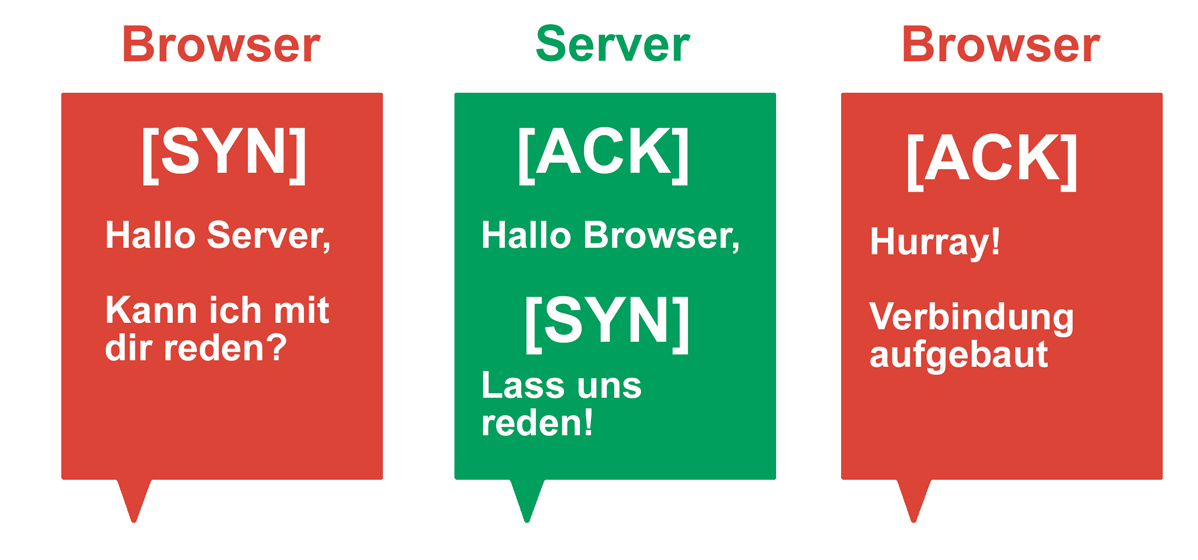
\includegraphics[width=0.6\textwidth]{three_way_handshake.jpg}
				\caption{Three-Way-Handshake zum Aufbau einer TCP Verbindung zwischen Browser und Server (Eigene Abbildung nach: \autocite{bos})}
				\label{fig:three_way_handshake}
			\end{center}
		\end{figure}
	% subsection tcp_three_way_handshake (end)

	\subsection{Latenz} % (fold)
	\label{sub:latenz}
		Latenz bezeichnet die Verzögerung, bis ein Paket von Sender A zu Empfänger B gelangt ist.
	% subsection latenz (end)


	\subsection{Round Trip Time (RTT)} % (fold)
	\label{sub:round_trip_time_}
		"`Round Trip Time"' wird im Deutschen Paketumlaufzeit genannt. Es bezeichnet die Zeit die ein Datenpaket braucht um in einem Netzwerk von Sender A zu Empfänger B und wieder zurück zu gelangen. Bei einer Latenz von 100ms würde die RTT folglich 200ms betragen (Annahme: Hin- und Rückweg haben die selbe Zeit).
	
	% subsection round_trip_time_ (end)

	\subsection{TCP Slow Start} % (fold)
	\label{sub:tcp_slow_start}

		Ein Round Trip kann nicht beliebig viele Bytes transportieren sondern ist durch die sogenannte "`Congestion Window Size"'\footnote{engl. congestion: Stauung, Überlastung, Anhäufung} limitiert. Der Überbegriff für dieses Verhalten nennt sich "`Slow Start"'

		\begin{figure}[htbp]
			\begin{center}
				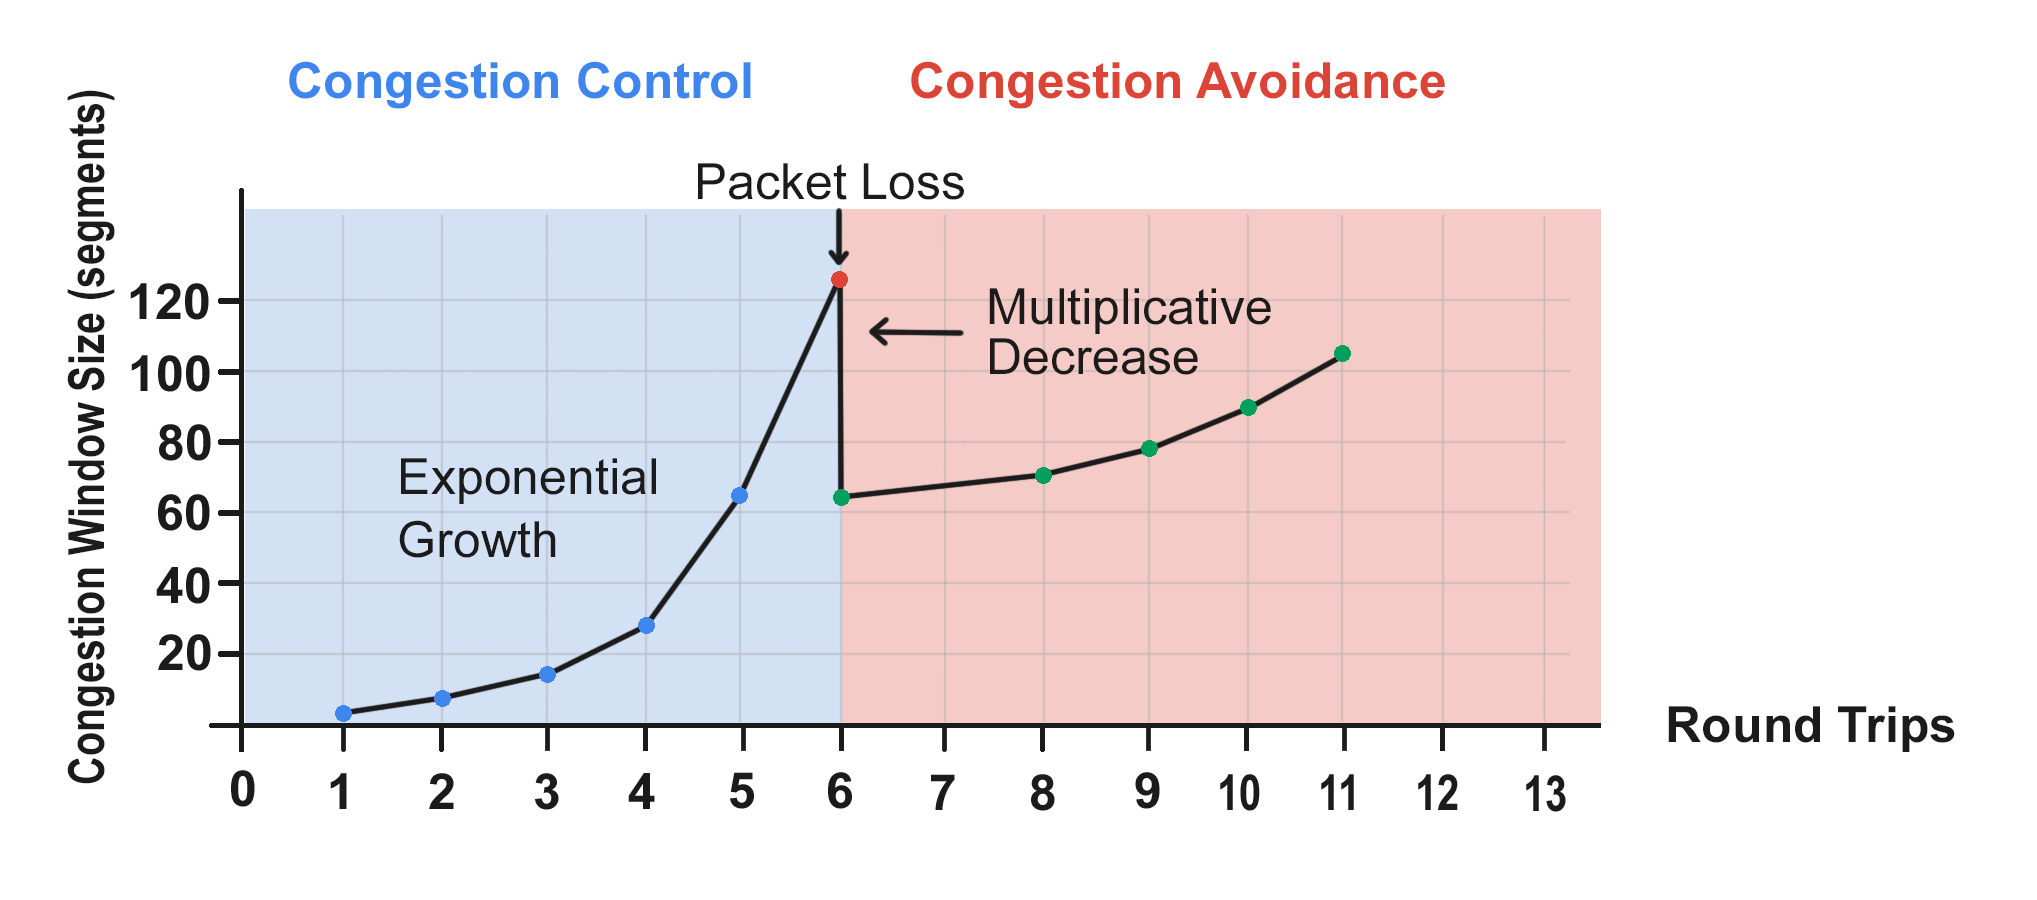
\includegraphics[width=\textwidth]{congestion_window_size.jpg}
				\caption{Congestion Control und Congestion Avoidance (Eigene Abbildung nach \autocite{grigorikSlowStart})}
				\label{fig:congestion_window_size}
			\end{center}
		\end{figure} 

		\begin{itemize}
			\item Congestion Control: Nach dem eine neue Verbindung per TCP aufgebaut wurde, können weder Server noch Client wissen, wie schnell die Verfügbare Bandbreite ist, mit der Daten ausgetauscht werden können. Um das Netzwerk, vor einem Datenstau zu schützen, wird mit einem sehr niedrigen Wert begonnen, der dann ansteigt bis das Limit erreicht ist. Dieses Verhalten nennt sich auch "`Congestion Control"' und verhindert das Aufstauen von Daten.
			\item Congestion Window Size: Diese Größe bestimmt, wieviel Bytes der pro Segmente geschickt werden darf, bis diese vom Empfänger per \texttt{ACK} (acknowledgement) bestätigt werden müssen. Die Größe der Segmente ist Standardmäßig 1460 bytes und die Rate bis zum ACK ist im April 2013 von 4 auf 10 Segmente erhöht worden.\autocite{grigorikSlowStart}. In der Grafik wird davon ausgegangen, das der erste Round Trip 4 Segmente senden darf. Die Datenrate Wächst exponentiell an, damit möglichst schnell die volle Bandbreite nutzbar ist.\\
			\item Congestion Avoidance bedeutet, dass sich die Datenrate wieder um ein Vielfaches verringert, falls es zu einem Paketverlust kommt. Da es besonders bei WLAN oder Mobilfunknetzen des öfteren zu Packetverlusten kommen kann ist dieser Aspekt besonders hervorzuheben, denn er verzögert das erreichen der maximal möglichen Datenrate.
		\end{itemize}

		Slow Start bedeutet also aus sicht der Performance, dass bei einer neuen TCP Verbindung nicht die maximale Bandbreite zu Verfügung steht. Bei größeren Dateien wird zwar durch das exponentielle Wachstum das Maximum schnell erreicht, gerade aber bei kleineren Dateien mit wenigen Kilobyte ist dies oft nicht der Fall.

	% subsubsection tcp_slow_start (end)

	\subsection{Http/1.1}
	\label{sub:http_1_1}
	
	% subsection http_1_1 (end)


	\subsection{Content Delivery Network (CDN)} % (fold)
	\label{sub:content_delivery_network}
		Ein Content Delivery Network (CDN), oder auch Content Distribution Network genannt, ist ein Netz lokal verteilter und über das Internet verbundener Server, mit dem Inhalte ausgeliefert werden.\\
		CDN-Knoten sind auf viele Orte verteilt um Anfragen (Requests) von End-Nutzern nach Inhalten (Content) möglichst ökonomisch zu bedienen.\\
		Große CDNs unterhalten tausende Knoten mit zehntausenden Servern.\autocite{wikipediaCDN}

		\begin{figure}[htbp]
			\begin{center}
				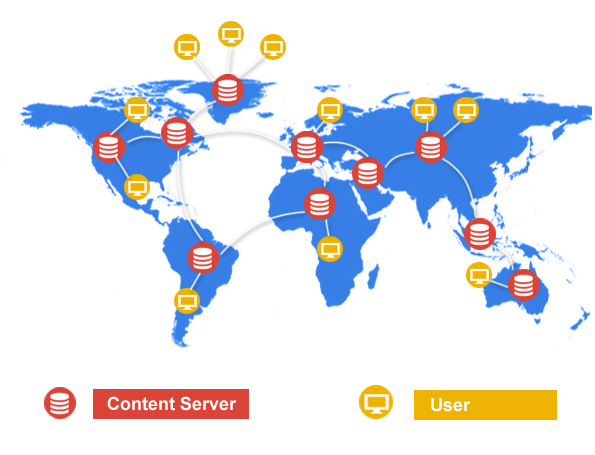
\includegraphics[width=0.6\textwidth]{cdn_network.jpg}
				\caption{Schematische Darstellung eines CDN (Eigene Abbildung nach \autocite{ritz14})}
				\label{fig:cdn_network}
			\end{center}
		\end{figure}
		
	% subsection content_delivery_network (end)


	\subsection{Above The Fold} % (fold)
	\label{sub:above_the_fold}
		Damit ist der auf einem Bildschirm sichtbare Bereich vor dem Scrollen gemeint. Diesem Bereich wird eine besondere Wichtigkeit zugesprochen.
		\begin{figure}[htbp]
			\begin{center}
				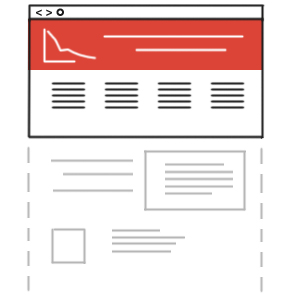
\includegraphics[width=0.3\textwidth]{above_the_fold.jpg}
				\caption{Darstellung des sichtbaren Bereichs vor dem Scrollen}
				\label{fig:above_the_fold}
			\end{center}
		\end{figure}

		\begin{quote}
			 \textit{"`In an analysis of 57,453 eyetracking fixations, we found that there was a dramatic drop-off in user attention at the position of the page fold. Elements above the fold were seen more than elements below the fold: the 100 pixels just above the fold were viewed 102\% more than the 100 pixels just below the fold."'} \autocite{nng15}
		\end{quote}

		Wichtige Informationen oder Navigationselemente sind meistens dort zu finden. Eine Webseite die nach dem Paradigma des Responsive-Webdesign aufgebaut ist kann dabei 3 oder mehrere Ansichten haben die alle einen unterschiedlichen "`above the fold"' bereich haben. Eine Anwendung kann aber auch unterschiedliche Seiten haben, auf dem der Anwender beim Aufrufen der Seite landen kann. Zum Beispiel wenn dieser An- oder Abgemeldet ist. Paradebeispiel dafür sind Facebook oder Twitter.

	% subsubsection above_the_fold (end)



	\subsection{Perceived Performance} % (fold)
	\label{sub:perceived_performance}
		\begin{figure}[htbp]
			\begin{center}
				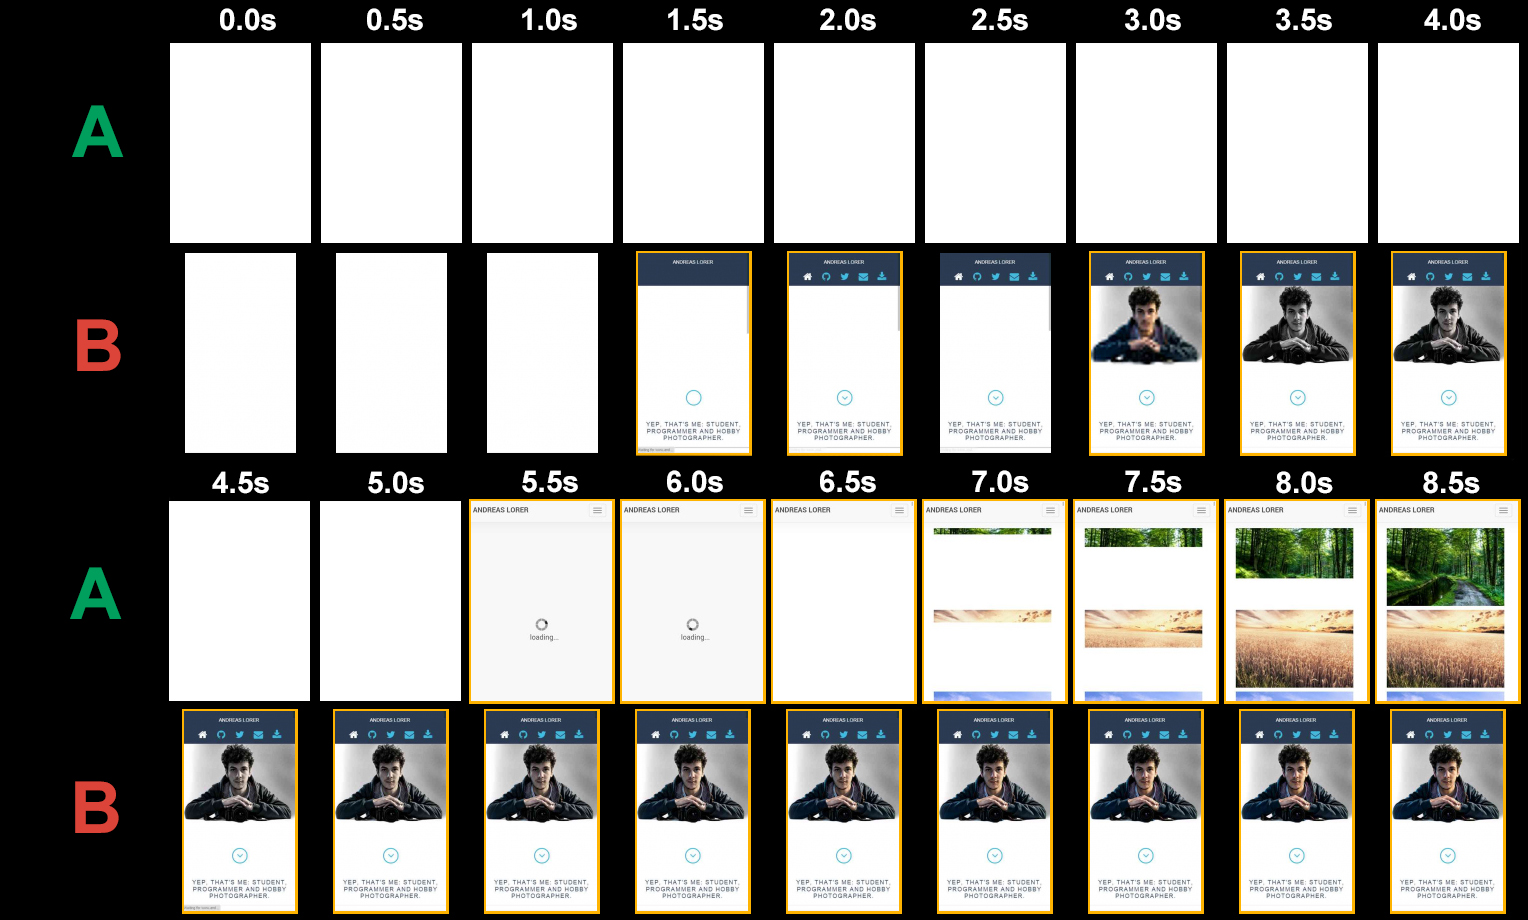
\includegraphics[width=0.9\textwidth]{perceived_performance.jpg}
				\caption{Zwei Seiten im Vergleich (Eigene Abbildung via webpagtest.org)}
				\label{fig:perceived_performance}
			\end{center}
		\end{figure}

		Abbildung \ref{fig:perceived_performance} zeigt die Seiten A und B, mit nahezu identischer Ladezeit. Der Unterschied besteht darin, dass Seite B bereits nach 1.5 Sekunden eine erste visuelles Rückmeldung für den Anwender zu sehen ist wohingegen Seite A erst nach 5.5 Sekunden dem Anwender zeigt, dass sie überhaupt ladet.
		"`Perceived Performance"' steht also für die Zeit bis ein erste visuelle Rückmeldung für den Anwender zu sehen ist und bedeutet, dass die Ladezeit als schneller empfunden wird, als es eigentlich laut Messwerten der Fall ist. Warum diese "`Perceived Performance"' für eine Webanwendung so wichtig ist zeigen mehrere Studien, deren Daten in folgender Infographik aufbereitet sind.

		\begin{figure}[htbp]
			\begin{center}
				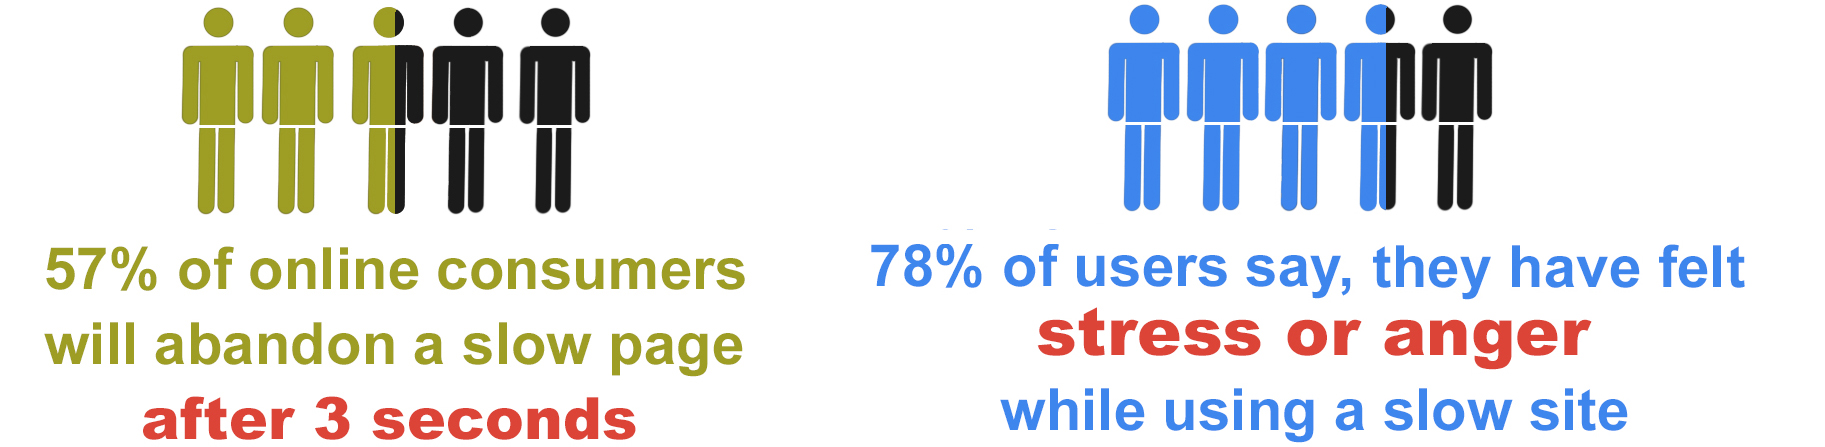
\includegraphics[width=0.7\textwidth]{effect_of_slow_loadtimes.jpg}
				\caption{Einfluss und Effekt einer langsamen Seite auf den Anwender (Eigene Abbildung nach Daten von: \autocite[p. 8]{radware14})}
				\label{fig:effect_of_slow_loadtimes}
			\end{center}
		\end{figure}

		Bereits kleine Verbesser- oder Verschlechterungen der Ladezeit können einen großen Einfluss in auf den Anwender haben. Yahoo hat herausgefunden, dass wenn eine Seite um nur 400 Millisikunden schneller ist, sich der Traffic um 9\% erhöhte.\autocite{stefanov08} 57\% der Online Konsumenten haben eine Seite, die länger als 3 Sekunden ladet bereits wieder verlassen. 78\% der Anwender empfinden sogar Zorn oder Stress wenn eine Seite nicht Ladet oder dies nicht ersichtlich ist.

	% subsubsection perceived_performance (end)
	\pagebreak
% subsection begriffe (end)



\section{Die 1000 ms Barriere} % (fold)
\label{sec:die_1000_ms_barriere}
	Das Ziel dieser Arbeit, die 1000 Millisekunden Barriere zu durchbrechen, wurde nicht durch einen Zufall gewählt. Der Anwender nimmt die Geschwindigkeit einer Seite subjektiv wahr. Sie wird in der folgenden Grafik interpretiert:

	\begin{figure}[htbp]
		\begin{center}
			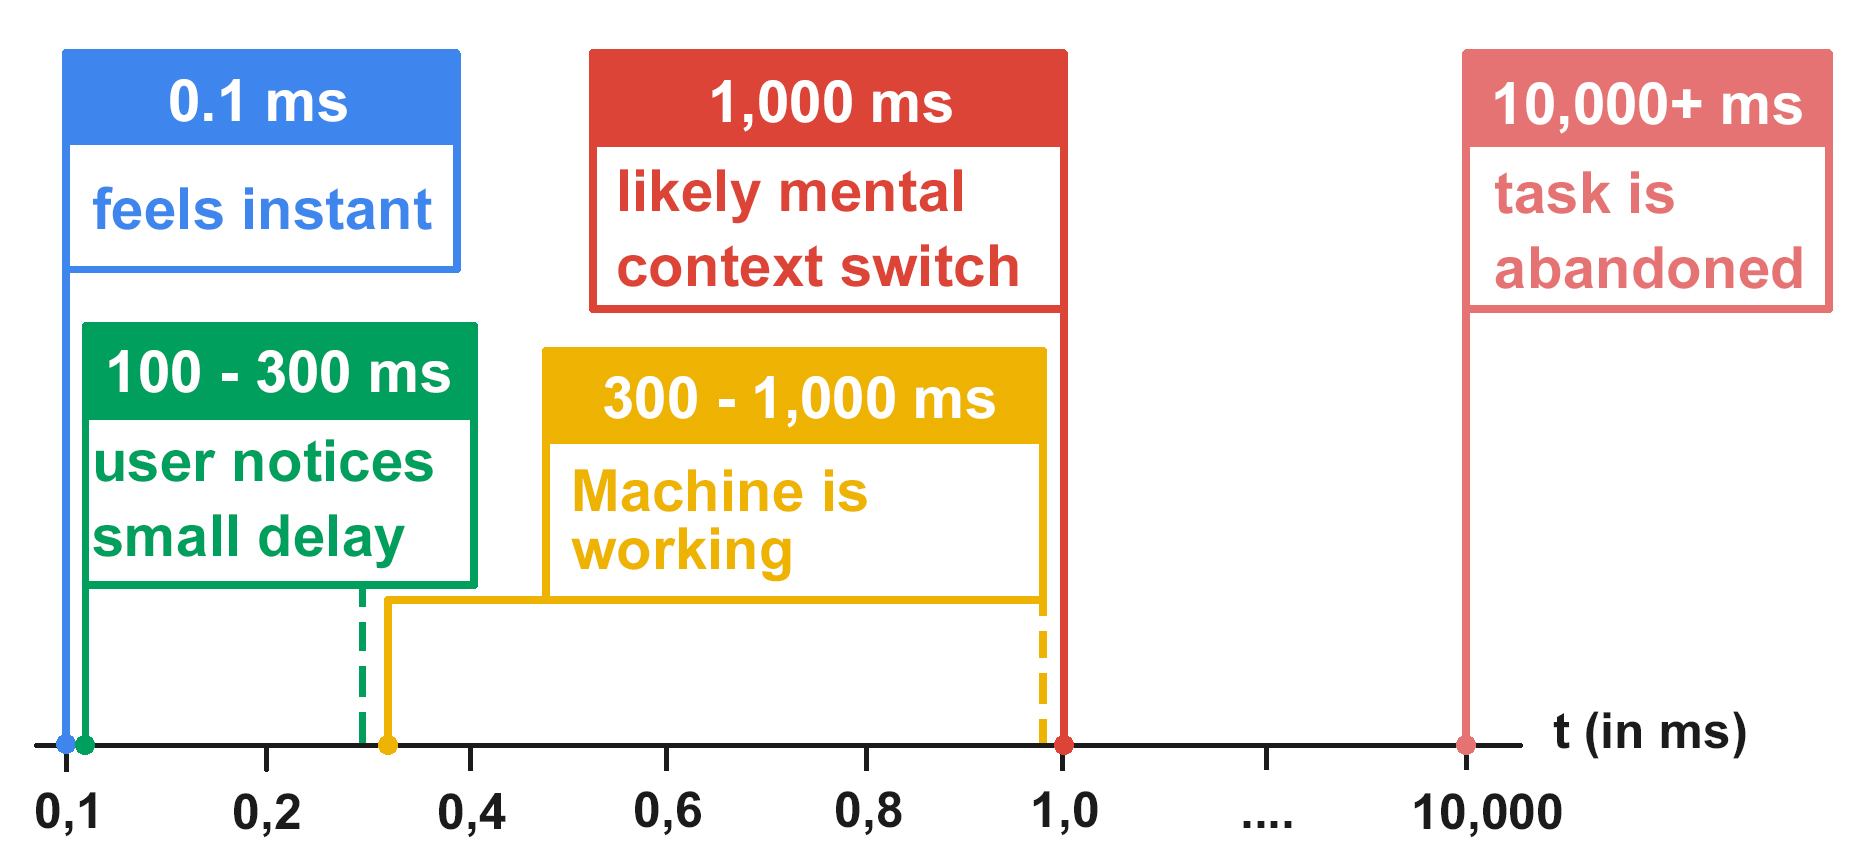
\includegraphics[width=\textwidth]{human_perception.jpg}
			\caption{Zeit und Wahrnehmung durch den Anwender (Eigene Abbildung nach Daten von: \autocite{grigorikHumanPerception})}
			\label{fig:human_perception}
		\end{center}
	\end{figure}

	Wie zu sehen ist bleiben gerade einmal eine Sekunde, bevor das Gehirn uns sagt, man solle doch einer anderen Aufgabe nachgehen bis der Ladevorgang abgeschlossen ist. Der Anwender verlangt visuelle Rückmeldung um "`am Ball zu bleiben"', dies wurde bereits in Punkt ~\ref{sub:perceived_performance} "`Perceived Performance"' angesprochen. Auf vielen Webseiten sieht man deshalb, Ladebalken oder sogenannte \texttt{Spinner}, die dem Anwender sagen, dass der Ladevorgang in gange, aber noch nicht abgeschlossen ist.

	Um das Ziel von einer Sekunde Ladezeit bis zum ersten Render zu erreichen, ist es nötig zu verstehen womit die meiste Zeit beim Aufrufen einer Webanwendung verbracht wird. Bevor eine Seite mittels Smartphone vom Browser dargestellt wird läuft eine ganze Reihe von Prozessen ab.



	\subsection{Touch Event} % (fold)
	\label{sub:touch_event}
		Der Aufruf einer Seite über das Smartphone erfolgt über ein Touch Event auf einen Link, Button oder die Seite wird per URL aufgerufen. Hierbei können je nach Gerät zwischen 50 (IPhone 5) und 123 Millisekunden (Moto X - Android) zwischen der Berührung des Touch Screen und dem Registrieren des Events vergehen.\autocite{venturebeat} Der Browser wartet allerdings nochmals bis zu 300 Millisekunden, denn er muss abwarten ob vielleicht noch ein zweiter Finger aufgelegt wird, oder ob der Anwender Scrollen oder Zoomen möchte.\autocite{google11}

		Dieses Verhalten lässt sich bei vielen Browsern per \texttt{Meta Tag} abstellen:

		\begin{lstlisting}
			<meta name="viewport" content="user-scalable=no">
		\end{lstlisting}

		Dies setzt natürlich voraus, dass die Webanwendung kein Zoomen benötigt um sie zu bedienen! Gerade bei älteren Webseiten trifft das oftmals nicht zu, da sie keine für das Smartphone angepasste Ansicht haben (responsive view). Eine vollständige Liste mit Meta Tags für die verschiedenen Browser ist der Fußnote zu entnehmen.\footnote{Suppressing 300ms delay for touchscreen interactions: \url{http://tinyurl.com/psj5nxz}}

	% subsection touch_event (end)

	\subsection{Netzwerke} % (fold)
	\label{sub:netzwerke}
		Warum gerade das nutzen des Internets per Smartphone so langsam sein kann (und oftmals ist) liegt zu einem Großteil am Netzwerk. Eine Studie untersuchte die Top eine Millionen Webseiten des Internets auf ihre Ladezeiten. Dabei wurde eine Verbindung von 5 Mbit/s und 28ms RTT benutzt. Eine RTT von 28 ms ist sehr schnell, vergleicht man sie zum Beispiel mit der Latenz des 3G Netzes (Abbildung ~\ref{fig:mobile_networks}). Diese Studie kam zu dem Ergebnis, dass fast 70\% der Ladezeit nur durch warten auf das Netzwerk verbracht wird:

		\begin{figure}[htbp]
			\begin{center}
				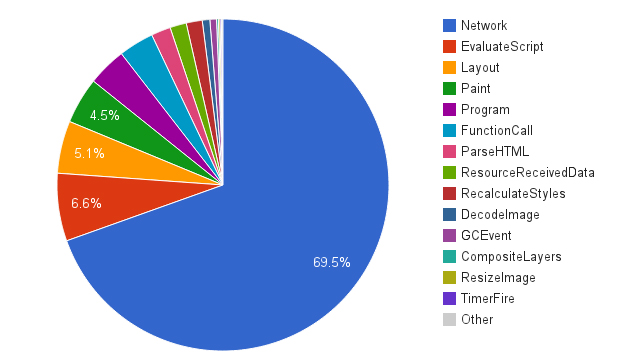
\includegraphics[width=0.8\textwidth]{time_on_network.jpg}
				\caption{Untersuchung der top 1 Millionen Alexa Seiten (Abbildung von: \autocite{alexa})}
				\label{fig:time_on_network}
			\end{center}
		\end{figure}

		Es macht also durchaus Sinn, sich diesen Bereich näher anzusehen, um zu verstehen worauf Einfluss genommen werden kann und wo nicht.


		\subsubsection{Mobilfunknetz} % (fold)
		\label{ssub:Mobilfunknetz}
			Es gibt unterschiedliche Mobilfunktsandards mit denen Anwender Anbindung an das Internet erlangen. Aber selbst wenn einem Anwender 4G vom Mobilfunkanbieter versprochen wird, so ist die Netzabdeckung mit 4G noch nicht vollständig deckend. Das bedeutet, dass der Anwender auf ein niedrigeres Netz wie zum Beispiel 3G ausweichen muss. Die verschiedenen Netzwerke unterscheiden sich entscheidend in ihrer Datenrate und vor allem in der Latenz. Folgende Tabelle gibt eine Übersicht:

			\begin{figure}[htbp]
				\begin{center}
					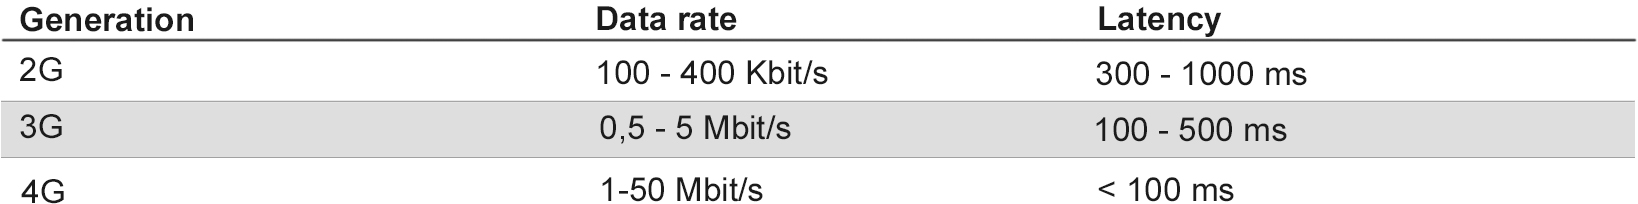
\includegraphics[width=\textwidth]{mobile_networks.jpg}
					\caption{Datenrate und Latenz für eine aktive mobile Verbindung (Eigene Abbildung nach Tabelle \autocite{grigorikGNetwork})}
					\label{fig:mobile_networks}
				\end{center}
			\end{figure}

			Unser Smartphone ist nicht ständig mit dem "`wireless service provider"' verbunden. Ist eine erste Verbindung nötig, so muss das Smartphone dem Sendeturm mitteilen, dass es Kommunizieren möchte. Der Anbieter muss die Anfrage Authentifizieren, die Verbindung herstellen und dann die Anfrage in das Internet weiter leiten. Die Zeit bis eine Authentifizierung erfolgt ist, kann je nach Anbieter und Mobilfunkstandard zwischen <100ms (LTE) und 2,5 Sekunden (3G) liegen \autocite{grigorikRadio}! Bereits hier ist zu sehen, dass es "`worst case"' Szenarien gibt, durch die es nicht möglich sein kann, dass eine Webanwendung unter einer Sekunde eine Rückmeldung gibt. Gerade Mobilfunknetze unterliegen Stoßzeiten, die Funksignale von Smartphones können sich gegenseitig stören oder das Signal kann in gewissen Gegenden stärker oder schwächer sein.

		% subsubsection Mobilfunknetz (end)


		\subsection{Der HTTP-Request} % (fold)
		\label{sub:der_http_request_komponente}
			Nachdem uns unser Mobilfunkanbieter mit dem Internet verbunden hat, kann die eigentliche Anfrage an den Server gestellt werden.

			\begin{figure}[htbp]
				\begin{center}
					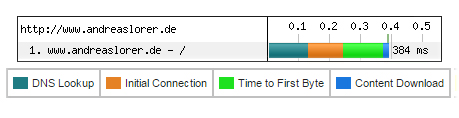
\includegraphics[width=0.8\textwidth]{http_components.jpg}
					\caption{Anfrage der HTML-Datei von Irland mittels 3G Netz (Abbildung nach \url{http://webpagetest.org})}
					\label{fig:http_components}
				\end{center}
			\end{figure}

			\begin{itemize}
				\item DNS Lookup: Um eine Verbindung mit dem Server herzustellen benötigt das HTTP Protokoll die IP Adresse des Ziels. Das heißt der DNS Server wird für den Namen "`http://andreaslorer.de"' die zu diesem Namen zugehörige IP Adresse zurückgegeben.

				\item Initial Connection bezeichnet die Zeit die vergeht, bis eine neue Verbindung zum Server hergestellt wurde damit eine Kommunikation zwischen Browser und Server stattfinden kann. Hierbei findet der sogenannte TCP "`Three-Way-Handshake"' statt, der dafür einen Round Trip benötigt.

				\item TTFB: Ist die Abkürzung für "`Time to first byte"'. Dieser Begriff beschreibt die Zeit die vergeht, bis das erste Byte vom Server beim Browser ankommt. Der Server muss den Request erst zusammenstellen bevor er ihn versenden kann. Dafür werden unter umständen Daten aus der Datenbank abgefragt oder es müssen berechnungen stattfinden. Diese Faktoren beeinflussen die TTFB und kann optimiert werden (schnellerer Server, bessere Datenbankanbindung, Caching).

				\item Content Download: Die Zeit die benötigt wird bis die Datei vom Server Heruntergeladen wurde.

				\item Nachdem das HTML Dokument heruntergeladen wurde, muss es vom Browser noch gelesen und interpretiert werden. Diese Zeit taucht im Diagramm nicht auf.
			\end{itemize}
					
		% subsection http_request_komponente (end)
	% section netzwerke (end)

	\subsection{Das Herunterladen einer 40 KB Datei} % (fold)
	\label{sub:das_herunterladen_einer_40_kb_datei}

		Abbildung ~\ref{fig:fetching_40kb} zeigt Schematisch wie eine 40 KB Datei mittels einer neuen TCP Verbindung heruntergeladen wird. Sie soll verdeutlichen, wie vor allem die RTT eine entscheidende Rolle spielt und warum die Latenz die Geschwindigkeit einer Seite viel höher beeinflusst als die Bandbreite.

		\begin{figure}[htbp]
			\begin{center}
				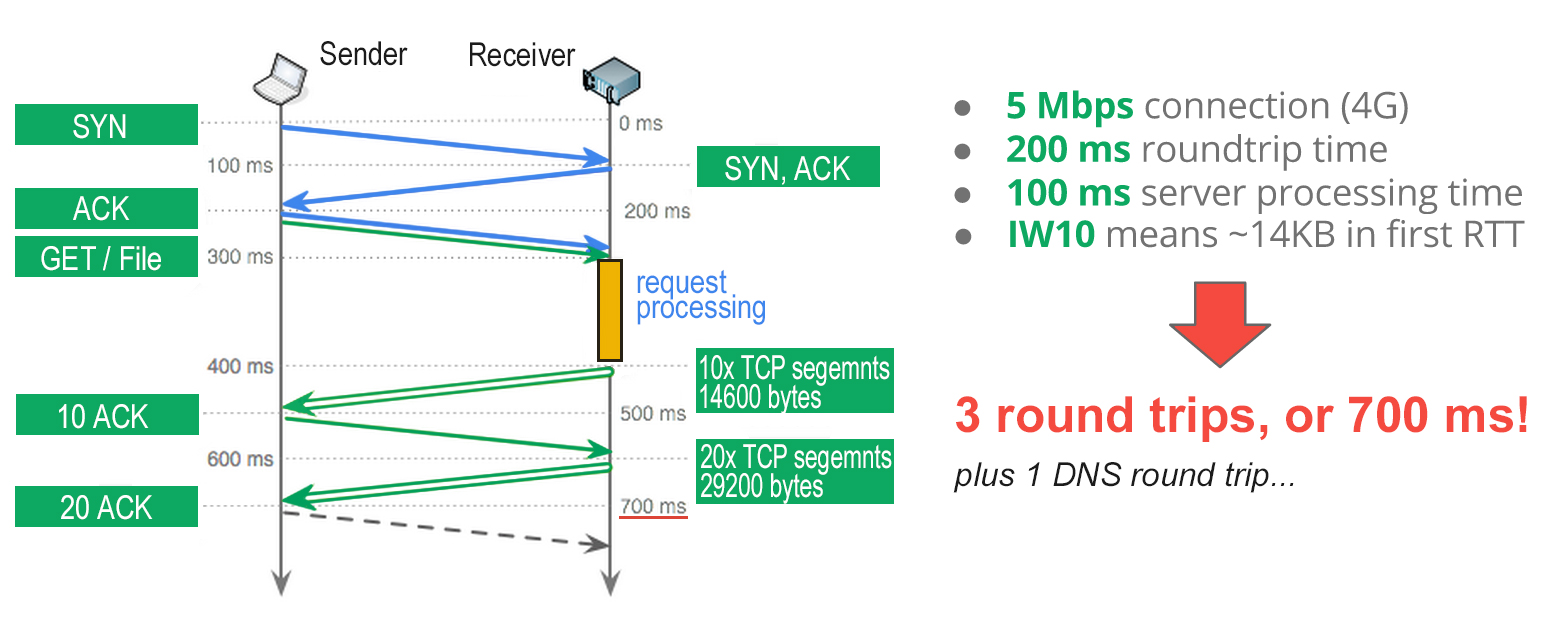
\includegraphics[width=\textwidth]{fetching_40kb.jpg}
				\caption{Herunterladen von 40KB mittels TCP (Abbildung nach \autocite{grigorikTCP})}
				\label{fig:fetching_40kb}
			\end{center}
		\end{figure}

		Zuerst erfolgt der DNS Lookup, dann muss TCP per \texttt{three way handshake} eine Verbindung aufbauen. Dies kostet bereits 2 round trips, was in diesem Beispiel 400 ms entspricht.
		Durch den TCP slow start (siehe Punkt: ~\ref{sub:tcp_slow_start} TCP slow start) steht bei einer neuen TCP Verbindung nicht die volle Bandbreite zur Verfügung. Deshalb kann die volle Datenmenge nicht auf einmal, sondern nur durch zusätzliche round trips heruntergeladen werden. Wenn die Performance einer Webanwendung verbessert werden soll, macht es also Sinn in round trips zu denken. Wieviel round trips sind nötig, bis ich dem Browser informationen übermittelt habe, so dass dieser etwas anzeigen kann? 
		
		\begin{figure}[htbp]
			\begin{center}
				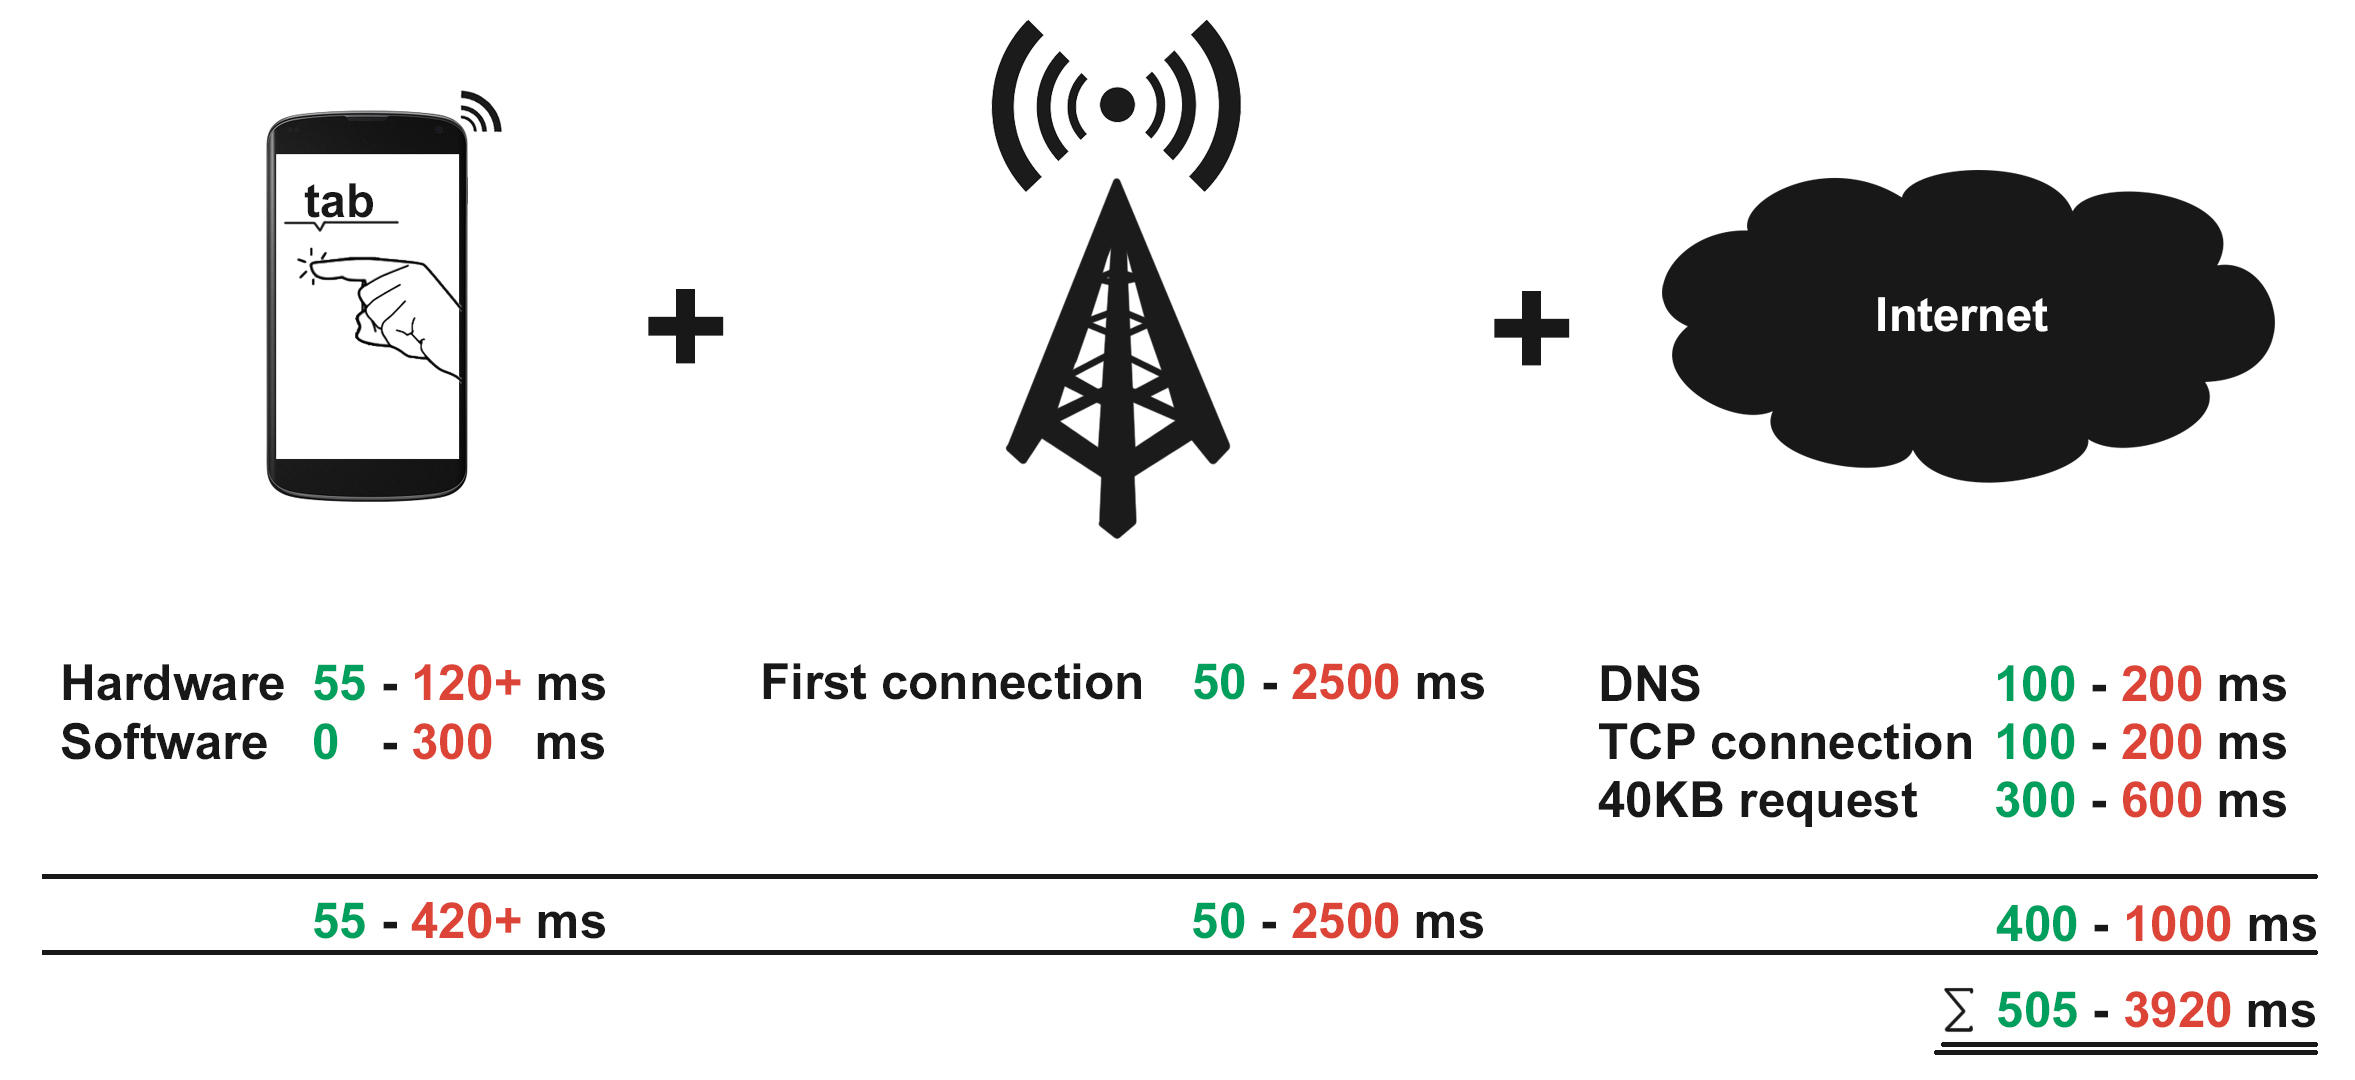
\includegraphics[width=0.9\textwidth]{1000ms_budget.jpg}
				\caption{1000 ms Budget (Eigene Abbildung)}
				\label{fig:1000ms_budget}
			\end{center}
		\end{figure}

		Wie in Abbildung ~\ref{fig:1000ms_budget} zu sehen ist bleibt von dem 1000 Millisekunden Budged nicht mehr viel übrig, wenn man alleine die Netzwerkzeiten abzieht. Im "`best case"' Szenario bleiben knapp 500 ms.
		Das bedeutet es müssen in den ersten Kilobytes, soviel nützliche Informationen vorhanden sein, damit der Browser bereits anfangen kann mit dem rendering zu beginnen, obwohl noch nicht alle Daten heruntergeladen sind. Noch spitzer formuliert: Der Browser sollte mit den ersten 14 KB (das ist die Menge an Daten die der erste round trip transportieren kann, siehe Abbildung ~\ref{fig:fetching_40kb}) bereits den \texttt{above the fold} bereich rendern können. Um das zu ermöglichen ist es nötig, den Kritischen Rendering-Pfad zu optimieren.
		
	% subsection das_herunterladen_einer_40_kb_datei (end)

	\subsection{Zusammengefasst} % (fold)
	\label{sub:zusammengefasst}
		Folgende Optimierungsmaßnahmen ergeben sich auf der Ebene des Netzwerks:
		\begin{itemize}
			\item Näheres Platzieren der Bits: Die Latenz bestimmt vorrangig die Geschwindigkeit des Ladevorgangs. Durch die benutzung eines CDN's lassen sich Bits und Bytes näher am Endanwender platzieren.
			\item Sage das Nutzerverhalten vorraus: Wenn der Anwender in einer Einkaufs-App 3 Schritte zum vollenden des Kaufvorgangs benötigt, dann lässt sich bei Schritt 1 bereits vorhersagen was er für weitere Ressourcen im nächsten Schritt benötigt. Diese Ressourcen könnten bereits geladen werden.
			\item Wahl eines guten Hostings: Die RTT als auch die \texttt{Server Response Time} sind je nach Anbieter unterschiedlich. Ein gutes Hosting kann hier unter umständen bereits eine enorme Verbesserung bedeuten. Zur not sollte gewechselt werden!

			\begin{figure}[htbp]
				\begin{center}
					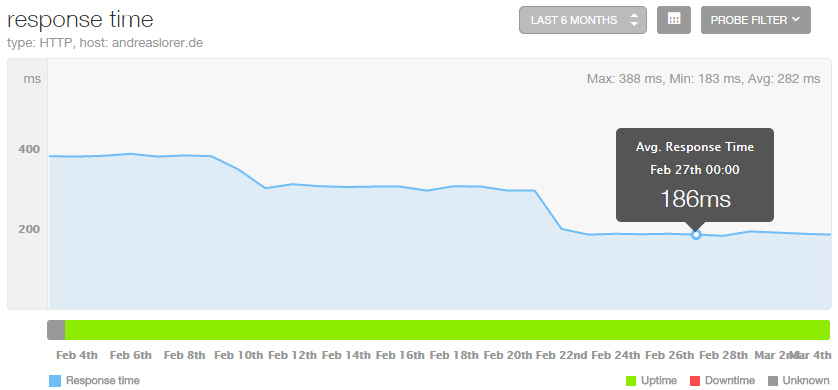
\includegraphics[width=0.9\textwidth]{choose_a_good_host.jpg}
					\caption{Verringerung der response time für http://andreaslorer.de (Abbildung nach pingdom.com)}
					\label{fig:choose_a_good_host}
				\end{center}
			\end{figure}
			
			Wie in der Grafik zu sehen ist, sank die Response Zeit meines Hosting Providers von durchschnittlichen fast 400 Millisekunden auf 183 ms. Dies kann mehrere Gründe haben, so kann sich das Routing zum Server geändert haben, der Server kann ein Update erhalten haben oder die Maschine kann gewechselt worden sein. Was letzten endes dazu geführt hat kann nicht gesagt werden.

			\item Senden von weniger Daten: Das schnellste Bit ist das, dass nicht gesendet wird. Das zusammenfügen und verkleinern von Javascript und CSS Dateien verringert die Dategröße. Zudem lassen sich die Daten per GZIP zwischen Browser und Server komprimieren. Wie dies Möglich ist wird später noch Konkretisiert.

			\item Vermeiden von Weiterleitungen: Abbildung ~\ref{fig:eliminate_redirects} zeigt den Seitenaufruf von hs-weingarten.de. Wie zu sehen ist, bekommen wir zwei mal einen HTTP 301 (Wert in Klammer) Response zurück: 

			\begin{quote}
				301 - Moved Permanently: \textit{"`Die angeforderte Ressource steht ab sofort unter der im "`Location"'-Header-Feld angegebenen Adresse bereit (auch Redirect genannt). Die alte Adresse ist nicht länger gültig."'} \autocite{wikipediaHTTP}
			\end{quote}

			\begin{figure}[htbp]
				\begin{center}
					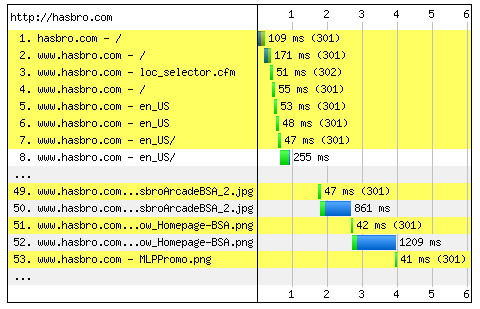
\includegraphics[width=\textwidth]{eliminate_redirects.jpg}
					\caption{Redirects verursachen große Verzögerungen (Abbildung nach webpagtest.org)}
					\label{fig:eliminate_redirects}
				\end{center}
			\end{figure}
			
			Wenn ein Anwender also hs-weingarten.de eingibt erfolgt der DNS Lookup und die TCP Verbindung wird aufgebaut nur um dann zu erfahren, dass die Ressource unter dieser Adresse nicht zur Verfügung steht. Danach erfolgt die DNS auflösung für www.hs-weingarten.de bei dem der gleiche Vorgang vonstatten geht. Es erfolgt die Weiterleitung auf www.hs-weingarten.de/web/willkommen/startseite.html mit wieder dem selben Vorgang.	Nach 855ms konnte die erste Anfrage an die richtige Zieladresse aufgegeben werden! Ruft man sich die RTT von einem 3G Netz ins Gedächtnis dürfte klar werden, was Weiterleitungen für den Smartphonenutzer bedeuten können. \\

			Die Weiterleitung von hs-weingarten.de auf www.hs-weingarten.de ist für die Suchmaschinenoptimierung \footnote{engl. SEO - search engine optimization} allerdings Sinnvoll, denn sonst würde unter zwei Namen der gleiche Inhalt zu finden sein. Dies ist aus sicht von Google "`Duplicated Content"' und kann zu einer Abstrafung im Ranking führen.\footnote{Mehr zu diesem Thema gibt es unter \url{http://www.sem-deutschland.de/seo-tipps/duplicate-content-definition/}}

		\end{itemize}

	% subsection zusammengefasst (end)
	\pagebreak



	\subsection{Kritischer Rendering-Pfad} % (fold)
	\label{sub:critical_render_path}
		Auf Englisch "`critical render path"' genannt, ist der wohl wichtigste Begriff, wenn es um schnelle Ladezeiten geht. Durch die Optimierung des Rendering Pfads kann die benötigte Zeit für das erste Rendern der Seite erheblich verkürzt werden. Das Verständnis des Rendering-Pfads ist zudem eine wesentliche Voraussetzung für die Erstellung von schnellen Webanwendungen und soll in diesem Abschnitt ausführlich erklärt werden. Dabei wird der Begriff in seine zwei Teile Zerlegt: Kritischer und Rendering-Pfad.\\

		Der \texttt{Rendering-Pfad} setzt sich aus den für die Anwendung nötige Ressourcen zusammen. Webanwendungen bestehen schließlich nicht nur aus einer HTML Datei, sondern aus mehreren Javascript und CSS Dateien.

		\begin{figure}[htbp]
			\begin{center}
				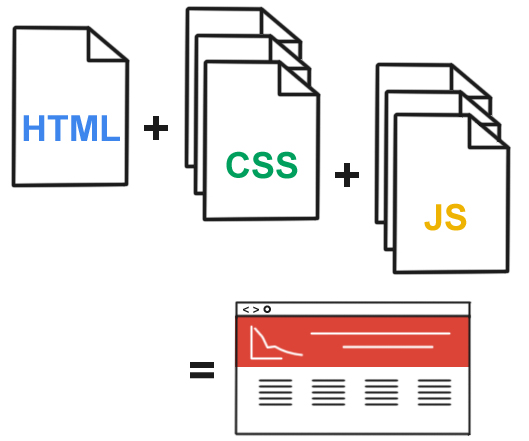
\includegraphics[width=0.4\textwidth]{critical_render_path.jpg}
				\caption{Ressourcen die für das Rendern von nöten sind (Eigene Abbildung)}
				\label{fig:critical_render_path}
			\end{center}
		\end{figure}

		Gegeben ist das folgende Beispiel einer simplen HTML Datei.

		\begin{lstlisting}
			<!DOCTYPE html>
			<meta charset="utf-8">
			<title>Web Performance fuer den mobilen Endanwender</title>

			<link href="assets/styles.css" rel="stylesheet" />
			<script src="assets/script.js"></script>

			<p> Hello world! </p>

		\end{lstlisting}

		Nachdem diese Datei heruntergeladen wurde, beginnt der Browser sie von oben nach unten zu lesen. Dabei stößt er in Zeile 5 auf einen \texttt{link tag} der ihn anweißt diese Datei herunterzuladen. In der nächsten Zeile findet der Browser einen \texttt{script tag}. Auch diese Datei muss herunterladen, interpretiert und ausgeführt werden, denn jede Javascript Datei kann den DOM-Baum oder das CSS manipulieren. Bevor also das "`Hello world"' in Zeile 8 angezeigt werden kann, ist das rendern blockiert. Dieses verhalten nennt sich auch "`Render Blocking"' und wird sowohl von Javascript als auch von CSS Dateien ausgelöst.	Erst dann kann der Browser mit dem rendern beginnen. Dieser Umstand erklärt auch warum die Regel gilt: CSS Dateien in den "`<head>"' und Javascript vor dem schließen des "`</body> tags"' zu platzieren.

		\begin{figure}[htbp]
			\begin{center}
				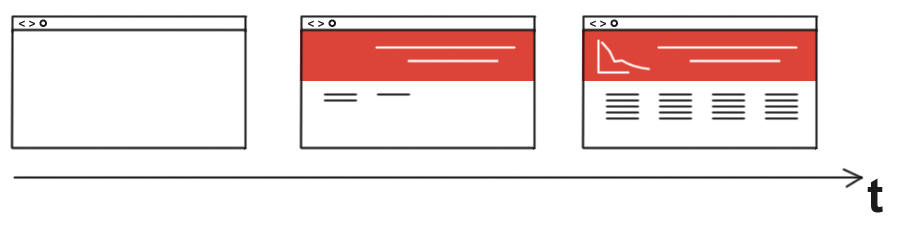
\includegraphics[width=0.75\textwidth]{browser_render.jpg}
				\caption{Der Render Prozess (Eigene Abbildung)}
				\label{fig:browser_render}
			\end{center}
		\end{figure}
	
		\texttt{Critical render path} sind genau die Javascript und CSS Dateien, die für den für das Rendern des \texttt{above the fold} von nöten sind. Um dies umzusetzen ist es nötig, die Ressourcen in zwei Teile zu zerlegen: Für das Rendering absolut notwendig und nicht notwendig. Alle Dateien die nicht notwendig für das erste Rendern sind sollten so lange mit dem Laden verzögert werden, bis die Anwendung geladen ist. Wie genau so eine Umsetzung aussieht, wird in Punkt: ~\ref{..} ausführlich gezeigt.

	% subsection critical_render_path (end)


	\subsection{Analyse des Wasserfalls}
	\label{sub:analyse_des_wasserfalls}
		Für ein besseres Verständnis des Kritischen Rendering-Pfads soll der stand meiner Webseite vor und nach den Performance Optimierungsmaßnahmen analyisiert werden. In Abbildung ~\ref{fig:wasserfall_old} ist ein Ausschnitt des Wasserfallmodell der nicht Optimisierten Webseite dargestellt. Das volle Diagramm ist der Fußnote \footnote{\url{http://www.webpagetest.org/result/150206_11_M2M/1/details/}} zu entnehmen.

		\begin{figure}[htbp]
			\begin{center}
				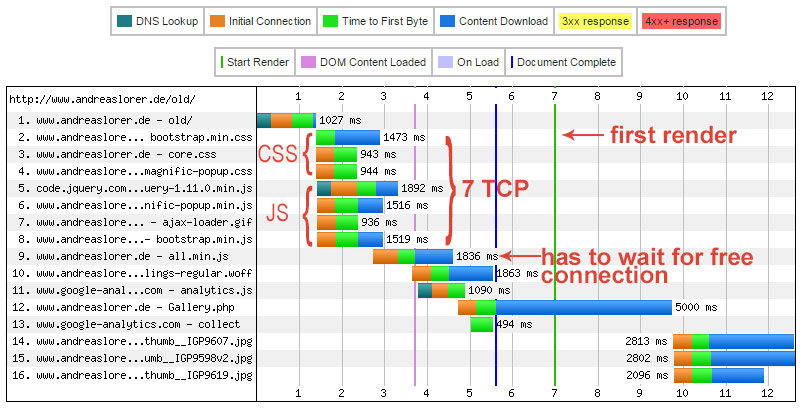
\includegraphics[width=\textwidth]{wasserfall_old.jpg}
				\caption{Ausschnitt des Wasserfallmodells der alten Seite (Eigene Abbildung nach webpagetest.org)}
				\label{fig:wasserfall_old}
			\end{center}
		\end{figure}
		
	  Die Abbildung zeigt, dass der Browser zuerst alle CSS und Javascript Dateien herunterläd. Hierbei fällt auf, dass er nicht mit allen gleichzeitig beginnen kann, sondern wie in Punkt ~\ref{sub:http_1_1}: HTTP/1.1 nur 6 TCP Verbindungen pro Hostname aufbauen darf. 

	% subsection analyse_des_wasserfalls (end)


% section die_1000_ms_barriere (end)


\pagebreak
